%
% $RCSfile: object_oriented_programming.tex,v $
%
% Copyright (C) 2002-2008. Christian Heller.
%
% Permission is granted to copy, distribute and/or modify this document
% under the terms of the GNU Free Documentation License, Version 1.1 or
% any later version published by the Free Software Foundation; with no
% Invariant Sections, with no Front-Cover Texts and with no Back-Cover
% Texts. A copy of the license is included in the section entitled
% "GNU Free Documentation License".
%
% http://www.cybop.net
% - Cybernetics Oriented Programming -
%
% http://www.resmedicinae.org
% - Information in Medicine -
%
% Version: $Revision: 1.1 $ $Date: 2008-08-19 20:41:07 $ $Author: christian $
% Authors: Christian Heller <christian.heller@tuxtax.de>
%

\subsection{Object Oriented Programming}
\label{object_oriented_programming_heading}
\index{Object Oriented Programming}
\index{OOP}
\index{Structured and Procedural Programming}
\index{SPP}
\index{Object Orientation}
\index{OO}
\index{Smalltalk}
\index{C++}
\index{C}
\index{Python}
\index{Common Lisp Object System}
\index{CLOS}
\index{Common Lisp}
\index{CL}
\index{Lisp}
\index{Class}
\index{Java}
\index{Unified Modeling Language}
\index{UML}
\index{UML Tool}

With the emerge of \emph{Object Oriented} (OO) languages, an additional
programming paradigm got introduced. That is, many principles such as
\emph{Structured and Procedural Programming} (SPP) were still holding true but
got extended through \emph{Object Oriented Programming} (OOP). Examples of OOP
languages, often defined by simply extending an existing language, are:

\begin{itemize}
    \item[-] \emph{Smalltalk} \cite{smalltalk}
    \item[-] \emph{C++}, extending the \emph{C} system programming language
        (section \ref{system_programming_heading})
    \item[-] \emph{Python}, as typeless programming language
        (section \ref{typeless_programming_heading})
    \item[-] \emph{Common Lisp Object System} (CLOS), extending the
        \emph{Common Lisp} (CL)\\dialect of the \emph{Lisp} functional
        programming language (section \ref{functional_programming_heading})
\end{itemize}

The following sections describe the main concepts behind OOP in brief. Although
many of them represent improvements to SPP, this work will point out their
weaknesses, too. The merger of attributes (data) and methods (operations) into
one common data structure called \emph{Class}, for example, will be criticised
and eliminated later in this work (chapter \ref{state_and_logic_heading}).

Code examples in the \emph{Java} programming language are given as well as
\emph{Unified Modeling Language} (UML) diagrams. The UML is a semi-formal,
graphical description language that offers elements for the concepts of
\emph{Object Orientation} (OO). To some extend, programs can be designed,
generated and documented using special applications called \emph{UML Tools}.

%
% $RCSfile: classification.tex,v $
%
% Copyright (C) 2002-2008. Christian Heller.
%
% Permission is granted to copy, distribute and/or modify this document
% under the terms of the GNU Free Documentation License, Version 1.1 or
% any later version published by the Free Software Foundation; with no
% Invariant Sections, with no Front-Cover Texts and with no Back-Cover
% Texts. A copy of the license is included in the section entitled
% "GNU Free Documentation License".
%
% http://www.cybop.net
% - Cybernetics Oriented Programming -
%
% http://www.resmedicinae.org
% - Information in Medicine -
%
% Version: $Revision: 1.1 $ $Date: 2008-08-19 20:41:05 $ $Author: christian $
% Authors: Christian Heller <christian.heller@tuxtax.de>
%

\subsubsection{Classification}
\label{classification_heading}
\index{Classification}
\index{Class}
\index{Attribute}
\index{Method}
\index{Structured Data Type}
\index{Struct}
\index{Record}
\index{Structured and Procedural Programming}
\index{SPP}
\index{Java}
\index{Global Variable}
\index{Instance}
\index{Object}
\index{Instantiation}
\index{Abstract Class}
\index{Interface}
\index{Inner Class}
\index{Bundling of Attributes and Methods}

The main idea of object oriented programming is to structure program code into
\emph{Classes} owning \emph{Attributes} and \emph{Methods} (figure
\ref{classification_figure}). They are comparable to the structured data types
(\emph{struct}, \emph{record}) of \emph{Structured and Procedural Programming}
(SPP) (section \ref{structured_and_procedural_programming_heading}) that can
own fields representing properties, but not behaviour. A class definition in
\emph{Java} source code looks like this:

\begin{scriptsize}
    \begin{verbatim}
    public class Example {
        private Type attribute;
        public void method(Type parameter) {
        }
    }
    \end{verbatim}
\end{scriptsize}

\begin{figure}[ht]
    \begin{center}
        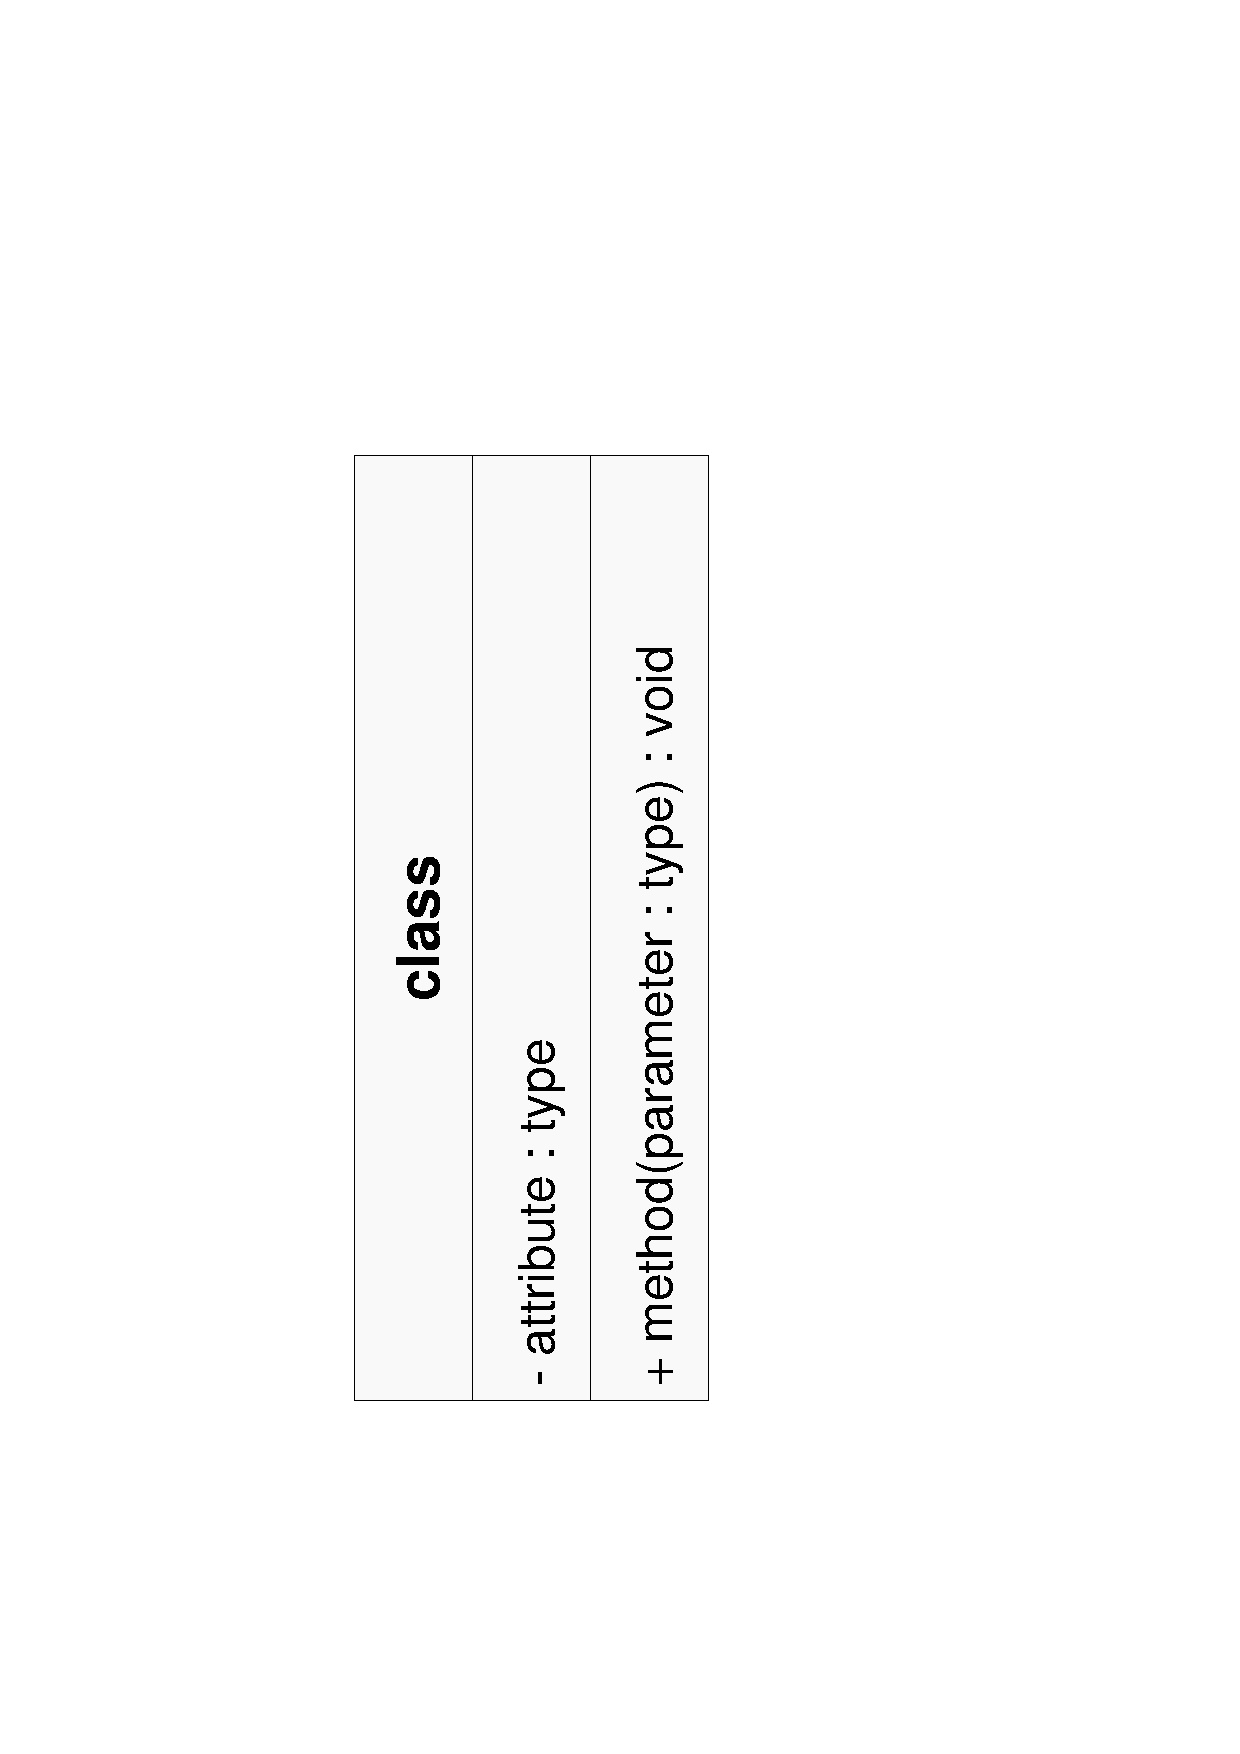
\includegraphics[scale=0.3,angle=-90]{graphic/classification.pdf}
        \caption{Classification as UML Diagram}
        \label{classification_figure}
    \end{center}
\end{figure}

While procedures and many variables in SPP are global, that is only exist once,
classes are treated as types of which many \emph{Instances} (also called
\emph{Objects}) can be created, including attributes and methods. In OOP, such
memory allocation is called \emph{Instantiation}.

Two related data types are \emph{Abstract Class} and \emph{Interface}. An
abstract class can hold attributes and (partly abstract) methods. Just like
interfaces, abstract classes cannot be instantiated. An interface is yet more
restricted in that it can only have constants but not attributes and only
declarations but not actual implementations of methods. Interfaces are commonly
used to \cite{steppan}:

\begin{itemize}
    \item[-] Realise multiple inheritance (section \ref{inheritance_heading})
    \item[-] Encapsulate components (section \ref{interface_and_implementation_heading})
    \item[-] Pool common methods (section \ref{separation_of_concerns_heading})
\end{itemize}

Specialities like \emph{Inner Classes} \cite{java} with limited scope of
validity are of minor importance to the argumentation of this document and not
further explained here.

The \emph{Bundling} of attributes and methods (state and logic) causes more
system interdependencies and complications than were predictable. It is a big
disadvantage that affects all modern object-oriented systems. \cite{heller2004}
Certainly, the bundling stems from best intentions to receive cleaner code by
keeping not only attributes but also methods in a common module, such avoiding
\emph{wild} and \emph{global} procedures. But now, modules not only have to
refer to other modules for accessing their state data; the same is needed for
accessing their logic in form of method calls.

With OOP, the number of cross-relations between modules, and inter-dependencies
between system layers may rise dramatically. In reality, state- and logic
properties are two \emph{different} things that have to be kept in different
places! Both can have a similar, hierarchical structure but each is a concept on
its own, as chapter \ref{state_and_logic_heading} will show.

%
% $RCSfile: encapsulation.tex,v $
%
% Copyright (C) 2002-2008. Christian Heller.
%
% Permission is granted to copy, distribute and/or modify this document
% under the terms of the GNU Free Documentation License, Version 1.1 or
% any later version published by the Free Software Foundation; with no
% Invariant Sections, with no Front-Cover Texts and with no Back-Cover
% Texts. A copy of the license is included in the section entitled
% "GNU Free Documentation License".
%
% http://www.cybop.net
% - Cybernetics Oriented Programming -
%
% http://www.resmedicinae.org
% - Information in Medicine -
%
% Version: $Revision: 1.1 $ $Date: 2008-08-19 20:41:06 $ $Author: christian $
% Authors: Christian Heller <christian.heller@tuxtax.de>
%

\subsubsection{Encapsulation}
\label{encapsulation_heading}
\index{Encapsulation}
\index{Access Method}
\index{Java}
\index{Information Hiding}
\index{Data Hiding}
\index{public}
\index{protected}
\index{private}
\index{Delphi}
\index{published}

One recommendation of object oriented programming is that the properties of an
object created as instance of a class be protected through special
\emph{Access Methods} (figure \ref{encapsulation_figure}). A \emph{Java} code
example can be found below. The intention is not to expose class attributes to
other classes by minimising direct access to them and such to provide some
security by preventing illegal access to an object's interna. Therefore, this
paradigm is called \emph{Encapsulation} or \emph{Information-/ Data Hiding}.
Another advantage is that if an attribute changes its name, then only one place
in the code (the access method), instead of hundreds, needs to be updated.

\begin{scriptsize}
    \begin{verbatim}
    public class example_class {
        private Type attribute;
        public void set_attribute(Type a) {
            this.attribute = a;
        }
        public Type get_attribute() {
            return this.attribute;
        }
    }
    \end{verbatim}
\end{scriptsize}

\begin{figure}[ht]
    \begin{center}
        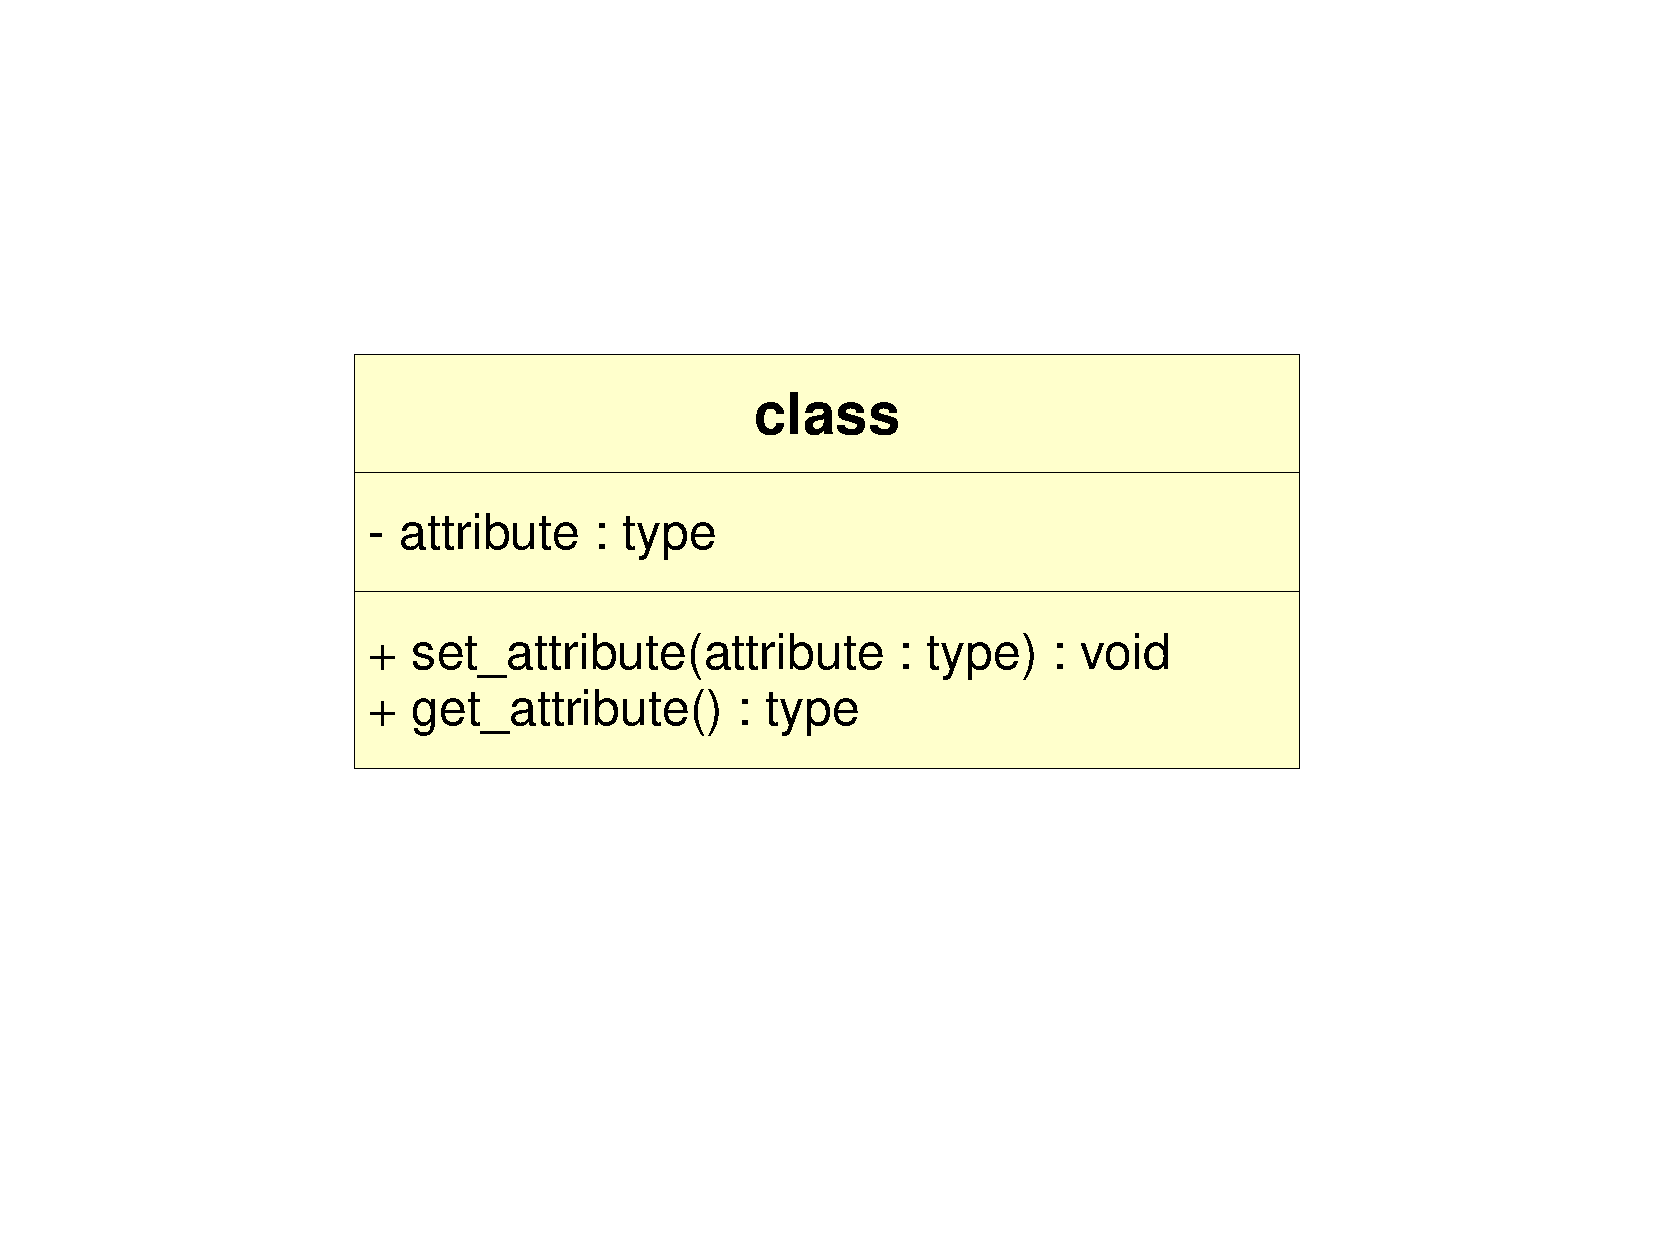
\includegraphics[scale=0.3,angle=-90]{graphic/encapsulation.pdf}
        \caption{Encapsulation as UML Diagram}
        \label{encapsulation_figure}
    \end{center}
\end{figure}

Special keywords are necessary to ensure proper encapsulation by making
attributes and methods \emph{visible} to only certain outside objects. These
keywords are: \emph{public}, \emph{protected} and \emph{private}. In the
\emph{Java} programming language \cite{java}, an additional package protection
level is applied when none of the aforementioned keywords is found. The
\emph{Delphi} language \cite{warken} knows an additional \emph{published}
keyword that makes properties visible in its object-inspector tool. Other
languages may contain further variations of access limitations.

The recommendation to encapsulate attributes produces thousands of lines of
source code whose usefulness is at least questionnable \cite{hellerbohl}. In
about 90\% of cases (practical experience of the author of this document), the
\emph{set} and \emph{get} methods consist of only one single line accessing an
attribute value which in the end is the same as accessing that attribute
directly. Sometimes, additional lines with a trigger function to update other
parts of the system are added. They get invoked whenever an attribute value of
the called object is changed by a \emph{set} method:

\begin{scriptsize}
    \begin{verbatim}
    public void set_attribute(Type a) {
        this.attribute = a;
        get_update_manager().update(this);
    }
    \end{verbatim}
\end{scriptsize}

But, as shown below, this update notification could as well be taken over by
the object that was calling the \emph{set} method:

\begin{scriptsize}
    \begin{verbatim}
    public void method() {
        example_object.set_attribute(a);
        get_update_manager().update(example_object);
    }
    \end{verbatim}
\end{scriptsize}

The argumentation that \textit{in this case a lot of redundant code would be
produced since the update function has to be implemented in every calling
object, instead of just once in the called object} does not really hold true
when looking into programming practice. The number of external objects calling
an object is mostly very well manageable. It finally seems that thousands of
\emph{set}/ \emph{get} access methods could be eliminated which would lead to a
tremendous code reduction and improved clearity.

The language introduced in chapter \ref{cybernetics_oriented_language_heading}
does not use encapsulation and the attributes (state knowledge) and methods
(logic knowledge) modelled in it are not bundled together.

%
% $RCSfile: inheritance.tex,v $
%
% Copyright (C) 2002-2008. Christian Heller.
%
% Permission is granted to copy, distribute and/or modify this document
% under the terms of the GNU Free Documentation License, Version 1.1 or
% any later version published by the Free Software Foundation; with no
% Invariant Sections, with no Front-Cover Texts and with no Back-Cover
% Texts. A copy of the license is included in the section entitled
% "GNU Free Documentation License".
%
% http://www.cybop.net
% - Cybernetics Oriented Programming -
%
% http://www.resmedicinae.org
% - Information in Medicine -
%
% Version: $Revision: 1.1 $ $Date: 2008-08-19 20:41:07 $ $Author: christian $
% Authors: Christian Heller <christian.heller@tuxtax.de>
%

\subsubsection{Inheritance}
\label{inheritance_heading}
\index{Inheritance}
\index{Superior Class}
\index{Parent Class}
\index{C++}
\index{Multiple Inheritance}
\index{Java}
\index{Single Inheritance}
\index{Interface}
\index{Application Programming Interface}
\index{API}

\emph{Inheritance} allows for code minimisation by letting classes inherit
attributes and methods from their \emph{superior} (sometimes called \emph{parent})
class (figure \ref{inheritance_figure}). Redundant code can such be avoided and
existing code can be reused. An inheriting class in \emph{Java} source code
looks like this:

\begin{scriptsize}
    \begin{verbatim}
    public class example extends super_class {
    }
    \end{verbatim}
\end{scriptsize}

\begin{figure}[ht]
    \begin{center}
        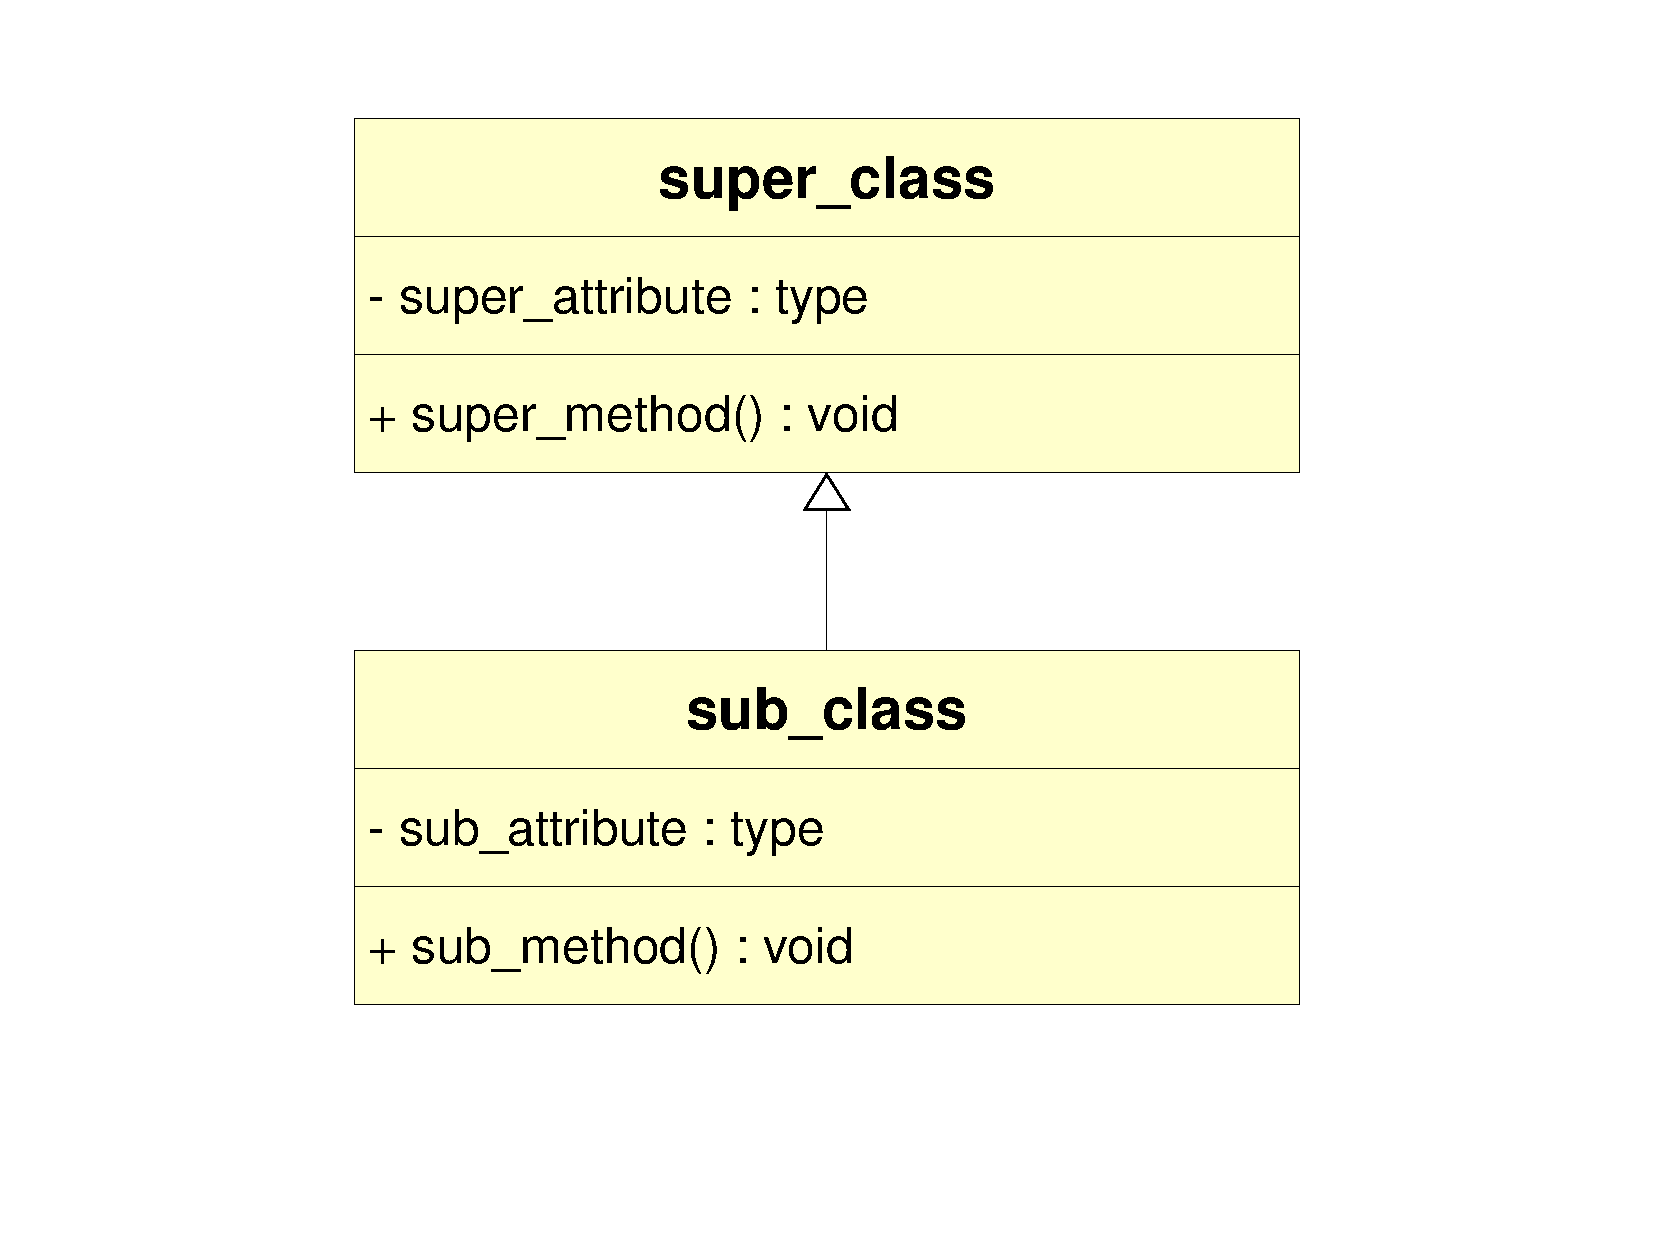
\includegraphics[scale=0.3,angle=-90]{graphic/inheritance.pdf}
        \caption{Inheritance as UML Diagram}
        \label{inheritance_figure}
    \end{center}
\end{figure}

Some object oriented programming languages (such as \emph{C++}) permit
\emph{Multiple Inheritance}. Classes written in those languages can have more
than one superior class. Other languages (such as \emph{Java}) that have
\emph{Single Inheritance} only, sometimes offer to \emph{inherit}
(\emph{realise}/ \emph{implement}) multiple interfaces. An interface forces its
subclasses to implement all methods it declares (more on this in section
\ref{interface_and_implementation_heading}) and can such provide a common
\emph{Application Programming Interface} (API) which makes classes
interchangeable and hence encourages reuse.

%
% $RCSfile: fragile_base_class.tex,v $
%
% Copyright (C) 2002-2008. Christian Heller.
%
% Permission is granted to copy, distribute and/or modify this document
% under the terms of the GNU Free Documentation License, Version 1.1 or
% any later version published by the Free Software Foundation; with no
% Invariant Sections, with no Front-Cover Texts and with no Back-Cover
% Texts. A copy of the license is included in the section entitled
% "GNU Free Documentation License".
%
% http://www.cybop.net
% - Cybernetics Oriented Programming -
%
% http://www.resmedicinae.org
% - Information in Medicine -
%
% Version: $Revision: 1.1 $ $Date: 2008-08-19 20:41:06 $ $Author: christian $
% Authors: Christian Heller <christian.heller@tuxtax.de>
%

\subsubsection{Fragile Base Class}
\label{fragile_base_class_heading}
\index{Fragile Base Class (Problem)}
\index{Implementation Inheritance}
\index{Subclass}
\index{Superclass}
\index{Class Hierarchy}
\index{Cascade of Change}
\index{Reusability}
\index{Flexibility}
\index{Cyclic Method Dependencies}
\index{Self-calling Assumptions of a Class Method}
\index{Base Class Access}
\index{Modifier Invariant Function}

Despite the possible code reduction through class inheritance, there are some
negative effects that hinder just this code reduction and reuse. John K.
Ousterhout writes in his article \cite{ousterhout1998}:

\begin{quote}
    Implementation inheritance, where one class borrows code that was written
    for another class, is a bad idea that makes software harder to manage and
    reuse. It binds the implementations of classes together so that neither
    class can be understood without the other: a subclass cannot be understood
    without knowing how the inherited methods are implemented in its superclass,
    and a superclass cannot be understood without knowing how its methods are
    inherited in subclasses. In a complex class hierarchy, no individual class
    can be understood without understanding all the other classes in the
    hierarchy. Even worse, a class cannot be separated from its hierarchy for
    reuse. Multiple inheritance makes these problems even worse. Implementation
    inheritance causes the same intertwining and brittleness that have been
    observed when goto statements are overused. As a result, object-oriented
    systems often suffer from complexity and lack of reuse.
\end{quote}

Unwanted dependencies caused simply by the usage of inheritance are called
\emph{Fragile Base Class Problem} \cite[section \emph{Layers}; p. 48]{buschmann}.
The source code changes resulting from base class manipulation are also called
\emph{Cascade of Change} \cite[Vorwort]{gruhn}. They are just the opposite of
what inheritance was actually intended to be for: \emph{Reusability}. Leonid
Mikhajlov and Emil Sekerinski \cite{mikhajlov} write:

\begin{quote}
    This problem occurs in open object-oriented systems employing code
    inheritance as an implementation reuse mechanism. System developers unaware
    of extensions to the system developed by its users may produce a seemingly
    acceptable revision of a base class which may damage its extensions.
    The fragile base class problem becomes apparent during maintenance of open
    object-oriented systems, but requires consideration during design.
\end{quote}

They identify the following \emph{Restrictions} \cite{mikhajlov} disciplining the
code inheritance mechanism, thus avoiding the \emph{Fragile Base Class Problem},
but on the cost of general \emph{Flexibility}:

\begin{itemize}
    \item[-] \emph{No cycles:} A base class revision and a modifier should not
        jointly introduce new cyclic method dependencies.
    \item[-] \emph{No revision self-calling assumptions:} Revision class methods
        should not make any additional assumptions about the behaviour of the
        other methods of itself. Only the behaviour described in the base class
        may be taken into consideration.
    \item[-] \emph{No base class down-calling assumptions:} Methods of a modifier
        should disregard the fact that base class self-calls can get redirected
        to the modifier itself. In this case bodies of the corresponding methods
        in the base class should be considered instead, as if there were no
        dynamic binding.
    \item[-] \emph{No direct access to base class state:} An extension class
        may not access the state of its base class directly, but only through
        calling base class methods.
    \item[-] \emph{No modifier invariant function:} A modifier should not bind
        values of its instance variables with values of the intended base class
        instance variables to generate an invariant.
\end{itemize}

In order to remain highly flexible and to avoid the fragile base class problem,
the language described in chapter \ref{cybernetics_oriented_language_heading}
does not use inheritance, although it could be extended to do so. In this case,
of course, its interpreter (chapter \ref{cybernetics_oriented_interpreter_heading})
would have to be adapted as well.

%
% $RCSfile: polymorphism.tex,v $
%
% Copyright (C) 2002-2008. Christian Heller.
%
% Permission is granted to copy, distribute and/or modify this document
% under the terms of the GNU Free Documentation License, Version 1.1 or
% any later version published by the Free Software Foundation; with no
% Invariant Sections, with no Front-Cover Texts and with no Back-Cover
% Texts. A copy of the license is included in the section entitled
% "GNU Free Documentation License".
%
% http://www.cybop.net
% - Cybernetics Oriented Programming -
%
% http://www.resmedicinae.org
% - Information in Medicine -
%
% Version: $Revision: 1.1 $ $Date: 2008-08-19 20:41:08 $ $Author: christian $
% Authors: Christian Heller <christian.heller@tuxtax.de>
%

\subsubsection{Polymorphism}
\label{polymorphism_heading}
\index{Polymorphism}
\index{Method Overloading}
\index{Method Overriding}
\index{Super Class}
\index{Sub Class}
\index{super}

Another object oriented feature that comes with inheritance is
\emph{Polymorphism}. It allows methods to be \emph{overloaded} (sometimes
called \emph{overridden}). That is, on two objects created from different
classes inheriting from each other, the right equally named method will be
called by the language interpreter program (figure \ref{polymorphism_figure}),
which leads to different behaviour depending on the current object context.
Following is a \emph{Java} code example overloading a method to gain
polymorphic behaviour:

\begin{scriptsize}
    \begin{verbatim}
    public class super_class {
        public void method() {
            do_something();
        }
    }
    public class sub_class extends super_class {
        public void method() {
            do_something_else();
        }
    }
    \end{verbatim}
\end{scriptsize}

\begin{figure}[ht]
    \begin{center}
        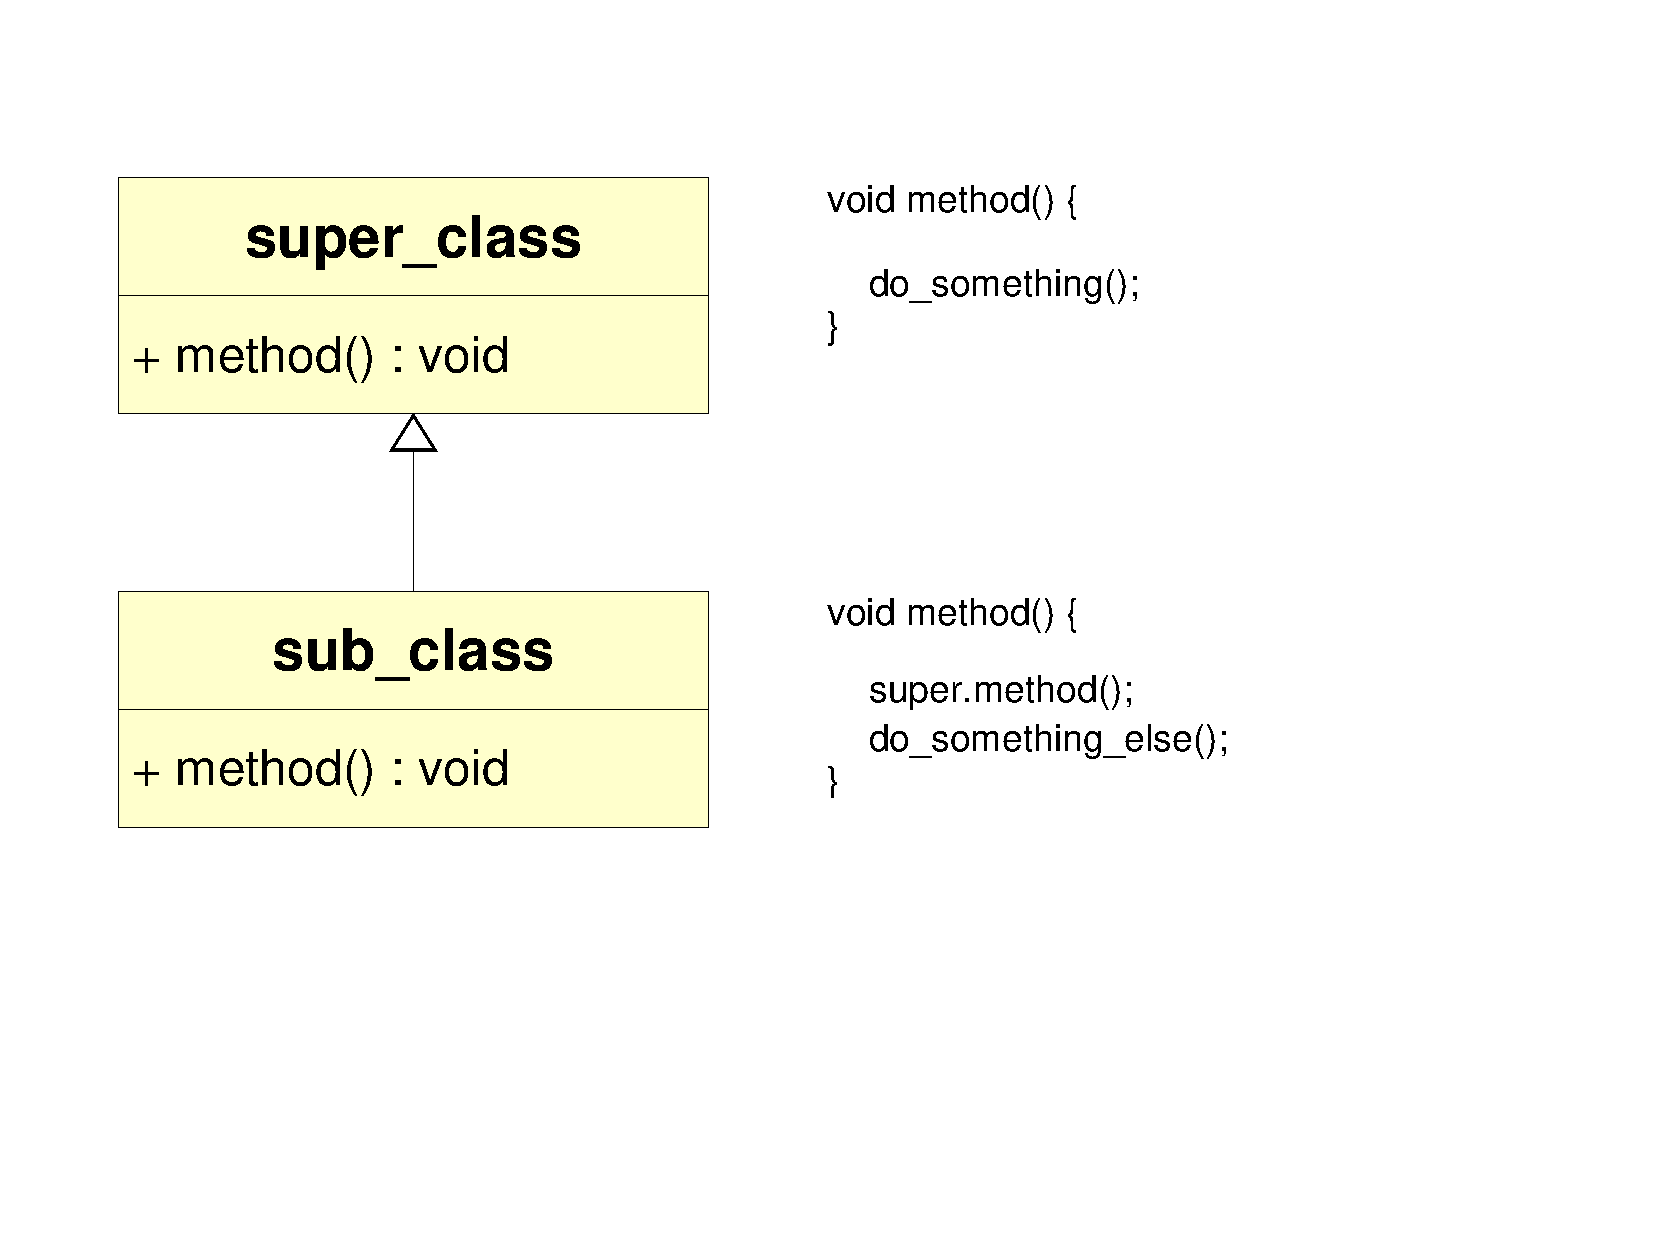
\includegraphics[scale=0.3,angle=-90]{graphic/polymorphism.pdf}
        \caption{Polymorphism as UML Diagram}
        \label{polymorphism_figure}
    \end{center}
\end{figure}

If objects instantiated from a sub class want to make use of the functionality
contained in the super class' equally named method, the sub class' method needs
to call the super class' method explicitly using the keyword \emph{super}:

\begin{scriptsize}
    \begin{verbatim}
    public class sub_class extends super_class {
        public void method() {
            super.method();
            do_something_else();
        }
    }
    \end{verbatim}
\end{scriptsize}

%
% $RCSfile: container.tex,v $
%
% Copyright (C) 2002-2008. Christian Heller.
%
% Permission is granted to copy, distribute and/or modify this document
% under the terms of the GNU Free Documentation License, Version 1.1 or
% any later version published by the Free Software Foundation; with no
% Invariant Sections, with no Front-Cover Texts and with no Back-Cover
% Texts. A copy of the license is included in the section entitled
% "GNU Free Documentation License".
%
% http://www.cybop.net
% - Cybernetics Oriented Programming -
%
% http://www.resmedicinae.org
% - Information in Medicine -
%
% Version: $Revision: 1.1 $ $Date: 2008-08-19 20:41:06 $ $Author: christian $
% Authors: Christian Heller <christian.heller@tuxtax.de>
%

\subsubsection{Container}
\label{container_heading}
\index{Container}
\index{Primitive Type}
\index{Java Container Framework}
\index{Collection}
\index{Map}
\index{Tree}
\index{Standard Template Library}
\index{STL}
\index{Sequence}
\index{Associative Container}

An object that got created through instantiating a class represents an
allocated area in a computer's memory which needs to be referenced in order to
be able to work with it, and to finally destroy it. The size of that area may
change \emph{dynamically}, depending on how the properties of the object are
manipulated. Primitive types like \emph{integer} or \emph{double} also reserve
memory space, only that the size of that space is \emph{not} dynamic; it is
pre-defined by the programming language, for each type. All
\emph{Structured- and Procedural Programming} (SPP) languages and some
\emph{Object Oriented Programming} (OOP) languages, like Java, offer standard
primitive types.

\begin{figure}[ht]
    \begin{center}
        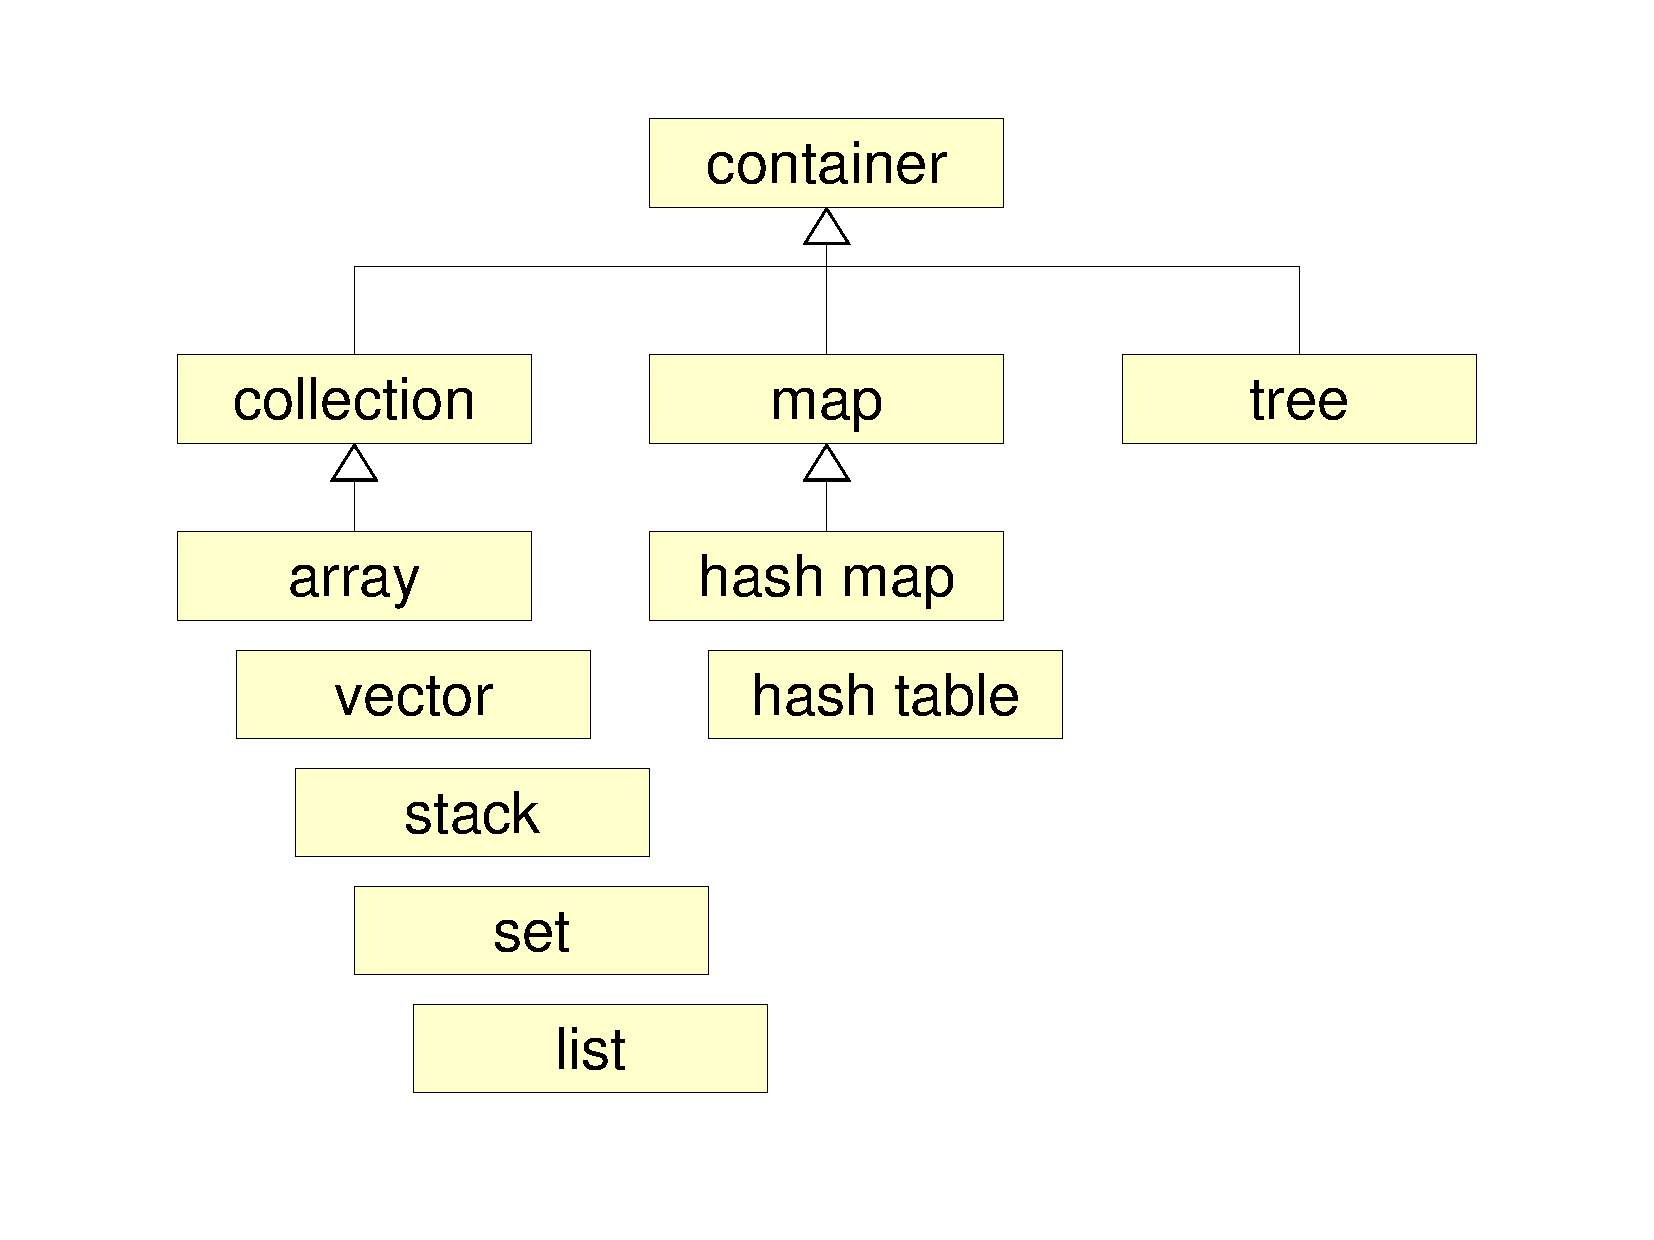
\includegraphics[scale=0.3,angle=-90]{graphic/container.pdf}
        \caption{Java Container Framework Systematics}
        \label{container_figure}
    \end{center}
\end{figure}

One way to store references to more than one dynamic element in memory, or
primitive data, is a \emph{Container}. Modern programming languages offer many
different kinds of containers. Figure \ref{container_figure} shows a
systematics of the Java container framework \cite{java}, as example, which gets
briefly introduced in the following paragraphs. Its main categories of
systematisation are \emph{Collection}, \emph{Map} and \emph{Tree}.

A similar library of container classes, algorithms and iterators exists for the
C++ programming language. It is called \emph{Standard Template Library} (STL)
\cite{stl} and it talks of \emph{Sequence} and \emph{Associative Container},
where Java says \emph{Collection} and \emph{Map}.

%
% $RCSfile: collection.tex,v $
%
% Copyright (C) 2002-2008. Christian Heller.
%
% Permission is granted to copy, distribute and/or modify this document
% under the terms of the GNU Free Documentation License, Version 1.1 or
% any later version published by the Free Software Foundation; with no
% Invariant Sections, with no Front-Cover Texts and with no Back-Cover
% Texts. A copy of the license is included in the section entitled
% "GNU Free Documentation License".
%
% http://www.cybop.net
% - Cybernetics Oriented Programming -
%
% http://www.resmedicinae.org
% - Information in Medicine -
%
% Version: $Revision: 1.1 $ $Date: 2008-08-19 20:41:05 $ $Author: christian $
% Authors: Christian Heller <christian.heller@tuxtax.de>
%

\paragraph{Collection}
\label{collection_heading}
\index{Collection}
\index{Array}
\index{Allocated Area}
\index{Random Access Memory}
\index{RAM}
\index{Vector}
\index{Stack}
\index{Last-In-First-Out}
\index{LIFO}
\index{Set}
\index{List}
\index{Duplicate Element}
\index{Ordered Collection}
\index{Sequence}
\index{Enumeration}
\index{nextElement Method}
\index{Java Development Kit}
\index{JDK}
\index{Iterator}

The \emph{Array} is the most basic form of a container. It represents an allocated
area in the computer's \emph{Random Access Memory} (RAM). A \emph{Vector}
implements a dynamically growable array of objects. The \emph{Stack} class extends
the vector class and represents a \emph{Last-In-First-Out} (LIFO) stack of objects.
A collection that contains no duplicate elements is called a \emph{Set}. Unlike
sets, \emph{Lists} typically allow duplicate elements. Synonyms for list are
\emph{Ordered Collection} and \emph{Sequence}.

Objects that can generate a series of elements, one at a time, implement the
\emph{Enumeration} interface. Successive calls to the \emph{nextElement} method
return successive elements of such a series. In recent releases of the
\emph{Java Development Kit} (JDK) \cite{java}, \emph{Iterator} takes the place
of enumeration, in the collections framework. An iterator over a collection
differs from an enumeration in that it allows the caller to remove elements,
with well-defined semantics, from the underlying collection during an iteration.

%
% $RCSfile: map.tex,v $
%
% Copyright (C) 2002-2008. Christian Heller.
%
% Permission is granted to copy, distribute and/or modify this document
% under the terms of the GNU Free Documentation License, Version 1.1 or
% any later version published by the Free Software Foundation; with no
% Invariant Sections, with no Front-Cover Texts and with no Back-Cover
% Texts. A copy of the license is included in the section entitled
% "GNU Free Documentation License".
%
% http://www.cybop.net
% - Cybernetics Oriented Programming -
%
% http://www.resmedicinae.org
% - Information in Medicine -
%
% Version: $Revision: 1.1 $ $Date: 2008-08-19 20:41:07 $ $Author: christian $
% Authors: Christian Heller <christian.heller@tuxtax.de>
%

\paragraph{Map}
\label{map_heading}
\index{Map}
\index{Dictionary}
\index{Table}
\index{Key-Value-Pair}
\index{Duplicate Key}
\index{Hash Map}
\index{Hash Table}
\index{Null Value}
\index{Null Key}

A \emph{Map} (also called \emph{Dictionary} or \emph{Table}) is an object that
maps \emph{Keys} to \emph{Values}. It cannot contain duplicate keys; each key
can map to at most one value. Java offers two kinds of a map: \emph{Hash Map}
and \emph{Hash Table}. The former is roughly equivalent to the latter, except
that it permits null values and the null key \cite{java, gumbel}.

%
% $RCSfile: tree.tex,v $
%
% Copyright (C) 2002-2008. Christian Heller.
%
% Permission is granted to copy, distribute and/or modify this document
% under the terms of the GNU Free Documentation License, Version 1.1 or
% any later version published by the Free Software Foundation; with no
% Invariant Sections, with no Front-Cover Texts and with no Back-Cover
% Texts. A copy of the license is included in the section entitled
% "GNU Free Documentation License".
%
% http://www.cybop.net
% - Cybernetics Oriented Programming -
%
% http://www.resmedicinae.org
% - Information in Medicine -
%
% Version: $Revision: 1.1 $ $Date: 2008-08-19 20:41:09 $ $Author: christian $
% Authors: Christian Heller <christian.heller@tuxtax.de>
%

\paragraph{Tree}
\label{tree_heading}
\index{Tree}
\index{Tree Node}
\index{Leaf Tree Node}
\index{Branch Tree Node}
\index{Root Tree Node}

A \emph{Tree}, or more exact \emph{Tree Node}, is a further kind of container.
Many tree nodes, in hierarchical order, may form a tree. A tree node may
represent a \emph{Leaf} with no children or a \emph{Branch} with one or more
children. The top-most tree node is usually called \emph{Root}.


%
% $RCSfile: falsifying_polymorphism.tex,v $
%
% Copyright (C) 2002-2008. Christian Heller.
%
% Permission is granted to copy, distribute and/or modify this document
% under the terms of the GNU Free Documentation License, Version 1.1 or
% any later version published by the Free Software Foundation; with no
% Invariant Sections, with no Front-Cover Texts and with no Back-Cover
% Texts. A copy of the license is included in the section entitled
% "GNU Free Documentation License".
%
% http://www.cybop.net
% - Cybernetics Oriented Programming -
%
% http://www.resmedicinae.org
% - Information in Medicine -
%
% Version: $Revision: 1.1 $ $Date: 2008-08-19 20:41:06 $ $Author: christian $
% Authors: Christian Heller <christian.heller@tuxtax.de>
%

\subsubsection{Falsifying Polymorphism}
\label{falsifying_polymorphism_heading}
\index{Falsifying Polymorphism}
\index{Container Inheritance}
\index{Hashtable}
\index{Copy Constructor}

Problems can occur when inheriting containers. This is now demonstrated on a Java
example adopted from \cite{javaiaq}.

\begin{figure}[ht]
    \begin{center}
        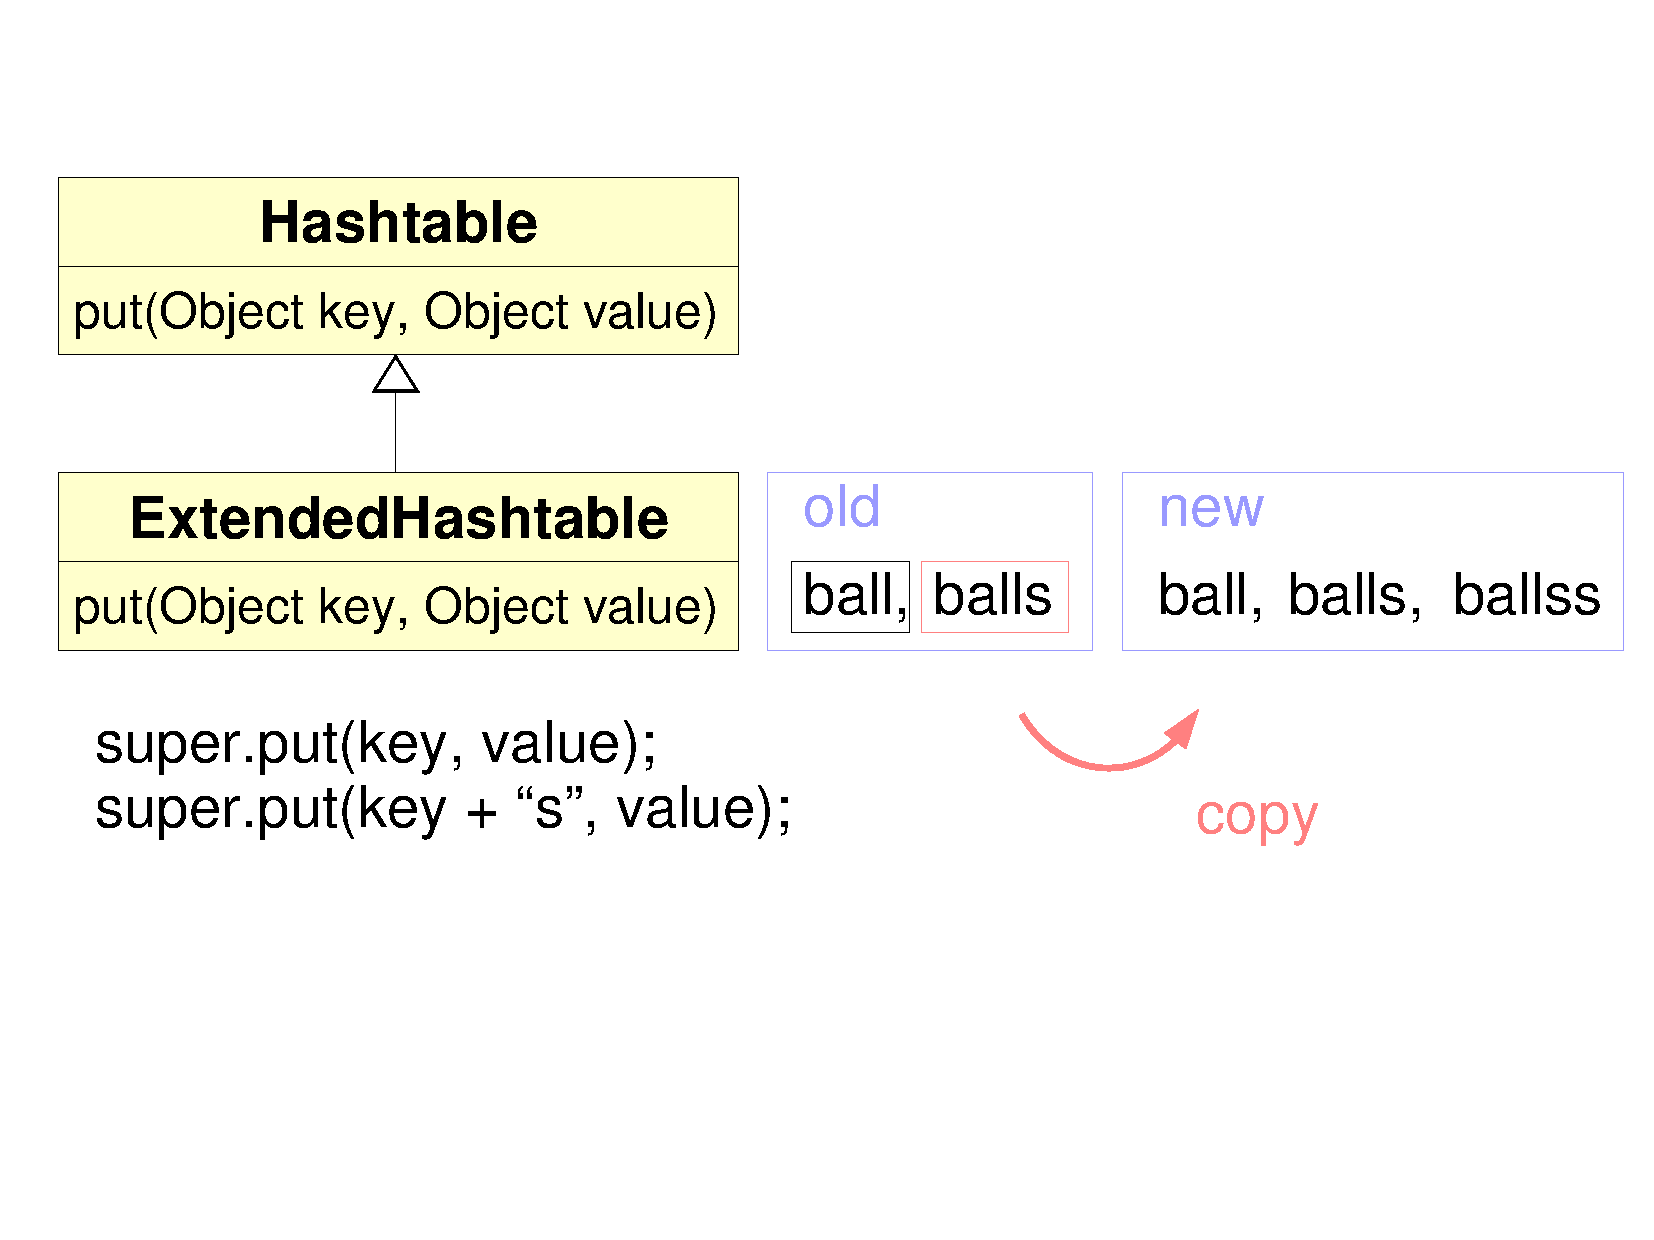
\includegraphics[scale=0.3,angle=-90]{graphic/falsifying.pdf}
        \caption{Falsified Contents with Container Inheritance}
        \label{falsifying_figure}
    \end{center}
\end{figure}

A class \emph{ExtendedHashtable} extends the standard container \emph{Hashtable}
(figure \ref{falsifying_figure}). The \emph{ExtendedHashtable} overrides the
\emph{put} method and lets it do two calls to the \emph{put} method of the
superior class \emph{Hashtable}, the second of these calls adding the letter
\emph{s} to the key.

A first object of type \emph{ExtendedHashtable} gets filled by calling the
\emph{put} method which adds two identical element values with the two different
keys \emph{ball} and \emph{balls} to the container. When the container is full,
a new one with extended size gets created and all values of the old have to be
copied into the new container, which is again of type \emph{ExtendedHashtable}.

If the \emph{put} method is now used to accomplish this, a falsified container
with more elements than the original one will be retrieved. The copying of the
first element \emph{ball} results in two elements \emph{ball} and \emph{balls},
placed in the new container. The copying of the second element \emph{balls} adds
two further elements \emph{balls} and \emph{ballss}, whereby the \emph{balls}
key stemming from the copying of the first element gets overwritten.

This example demonstrates only the principle of how the automatic size
extension of inherited container objects with element copying using
container-owned methods can incorrectly modify the container contents. The Java
language's \emph{Hashtable} class uses a slightly different mechanism, handing
over the hashtable object as parameter of a copy constructor which internally
calls a \emph{putAll} method which finally calls the \emph{put} method. Other
OOP languages may use different mechanisms. Of course, there are workarounds to
avoid the described troubles. But as a matter of fact, container inheritance
may -- due to polymorphism -- cause unpredictable behaviour leading to
\emph{falsified} container contents.

The language and interpreter introduced in chapters
\ref{cybernetics_oriented_language_heading} and
\ref{cybernetics_oriented_interpreter_heading} base on just one container
structure for knowledge representation, that covers many of the traditional
forms of containers.

%
% $RCSfile: conclusion.tex,v $
%
% Copyright (C) 2002-2008. Christian Heller.
%
% Permission is granted to copy, distribute and/or modify this document
% under the terms of the GNU Free Documentation License, Version 1.1 or
% any later version published by the Free Software Foundation; with no
% Invariant Sections, with no Front-Cover Texts and with no Back-Cover
% Texts. A copy of the license is included in the section entitled
% "GNU Free Documentation License".
%
% http://www.cybop.net
% - Cybernetics Oriented Programming -
%
% http://www.resmedicinae.org
% - Information in Medicine -
%
% Version: $Revision: 1.1 $ $Date: 2008-08-19 20:41:06 $ $Author: christian $
% Authors: Christian Heller <christian.heller@tuxtax.de>
%

\subsubsection{Conclusion}
\label{conclusion_heading}
\index{OOP Innovations}
\index{Object Oriented Programming}
\index{OOP}
\index{Structured and Procedural Programming}
\index{SPP}

As could be seen in the previous sections, OOP contributed many new concepts
to software design, thus trying to improve SPP. Most importantly, SPP data
structures (struct, record) got extended towards the \emph{Class} which does
not only hold data (attributes), but also operations (methods). This brought
with the concept of \emph{Encapsulation}, which permits only special methods of
an \emph{Object} (class instance) to access the data (properties) of that same
object. The next innovation was \emph{Inheritance}, which allows a class to
reuse the attributes and methods of its super class(es). Finally, inheritance
was used to introduce the concept of \emph{Polymorphism}, which lets objects
react differently, depending on the class they were instantiated with.

All of these concepts were true innovations as compared with traditional SPP
techniques. However, they have their own drawbacks: growth of the number of
dependencies within a system (links between classes), caused by the bundling of
attributes and methods; fragile base class problem; falsified container
contents with container inheritance. This work will not just revise these
concepts, but turn them upside down. Data (attributes) and operations/
algorithms (methods) are not bundled any longer; the resolution of inheritance
relationships at runtime gets eliminated and with it polymorphism; container
inheritance is not necessary any longer, since only one global container
structure (knowledge container) is used in a system. More on that in part
\ref{contribution_heading} of this work.

